\documentclass[conference]{IEEEtran}
\usepackage{amsmath,amssymb}
\usepackage{graphicx}
\usepackage{booktabs}
\usepackage{url}

\begin{document}

\title{An Interpretable Cascaded System for Blood-Cell Analysis and Hematological-Abnormality Screening}

\author{
\IEEEauthorblockN{C. Y. Samarasinghe (EG/2021/4775), H. M. S. Muthukumari (EG/2021/4685),\\
N. A. N. N. N. Arachchi (EG/2021/4408), and A. W. M. L. M. Bandara (EG/2021/4426)}
\IEEEauthorblockA{Department of Electrical and Information Engineering\\
University of Ruhuna, Galle, Sri Lanka}
}

\maketitle

\begin{abstract}
Microscopic examination of peripheral-blood smears is essential for cell counting and the recognition of hematological abnormalities, but manual review is time-consuming and subject to observer variability. This paper presents an interpretable, browser-accessible prototype for blood-smear analysis. The system uses a three-stage cascade: YOLOv8 detection first localizes red blood cells (RBCs), white blood cells (WBCs), and platelets; a WBC-crop classifier assigns neutrophil, lymphocyte, monocyte, and eosinophil labels; and a second crop classifier screens WBC crops across four acute-lymphoblastic-leukemia (ALL) severity classes. In parallel, contrast enhancement, marker-controlled watershed segmentation, and 22 morphological, colour, nuclear, and texture descriptors provide explainable measurements. Rule-based screening uses these measurements to flag patterns compatible with ALL, sickle-cell morphology, and anemia; the morphological basis for each rule is grounded in established hematological references, while the numerical thresholds remain engineering heuristics pending clinical validation. The evaluation protocol is stage-specific: detection is scored with precision, recall, and mAP at IoU 0.50 and 0.50:0.95; both crop classifiers are scored with per-class precision, recall, F1-score, a full confusion matrix, and the Matthews correlation coefficient (MCC); and segmentation is reported qualitatively in the absence of ground-truth masks. MCC is emphasized because it summarizes agreement over all confusion-matrix cells and is more robust than accuracy alone under class imbalance. On a group-aware, duplicate-free held-out split, Stage 1 detection reaches mAP@0.50 = 0.910 (precision 0.865, recall 0.883, $N=72$ images); Stage 2 WBC subtyping reaches 100.0\% accuracy and MCC = 1.00 ($N=2476$ crops); and Stage 3 ALL-severity screening reaches 99.84\% accuracy and MCC = 0.998 ($N=641$ crops). The near-perfect classification scores were verified to be free of source-level leakage, but are discussed critically rather than presented as clinical accuracy, since they most likely reflect the visual homogeneity of the public datasets used rather than real-world diagnostic performance. The system is an educational decision-support prototype, not a diagnostic medical device.
\end{abstract}

\begin{IEEEkeywords}
blood smear analysis, YOLOv8, white blood cell classification, watershed segmentation, Matthews correlation coefficient, interpretable computer vision
\end{IEEEkeywords}

\section{Introduction}

Blood-cell morphology and differential counts provide clinically useful evidence for hematological disorders. However, manual microscopic examination requires expertise and can be slow when many fields of view must be reviewed. Computer vision can assist by localizing cells, assigning cell types, measuring morphology, and presenting the evidence in a reproducible form.

This work develops a cascaded system rather than claiming a single model detects every cell type and disease state. Stage 1 detects RBCs, WBCs, and platelets in a full smear image. Stage 2 classifies each detected WBC crop into four subtypes. Stage 3 screens WBC crops using a separate leukemia classifier, which is the only disease flag learned from labelled disease data; sickle-cell and anemia flags are produced by a transparent, literature-informed rule layer over classical image features, since no cell-level ground truth for those two conditions was available for training a classifier. Classical image processing supplies interpretable cell measurements, while transparent rules generate screening flags. This separation matches the available data: full-smear data are suitable for localization, whereas the subtype and leukemia data consist of individual-cell images.

The contributions are:
\begin{itemize}
\item a working cascade that combines full-smear detection, WBC subtype classification, leukemia screening, and an interactive reporting interface;
\item watershed-based cell separation and a 22-feature morphology representation for explainable analysis, with each screening rule traced to a specific hematological reference rather than presented as a learned diagnostic decision;
\item a stage-specific verification protocol -- detection mAP/IoU, classification confusion matrices with MCC, and segmentation Dice -- so that every reported number matches the task it measures; and
\item an explicit account of dataset, validation, and clinical limitations.
\end{itemize}

\section{Related Work}

Deep detectors have been applied to blood-cell localization and counting, while cell-crop classifiers have been used for WBC subtyping. YOLOv8 offers a compact detector suitable for real-time prototype systems \cite{ref_yolo}. Detection quality in this class of problem is conventionally reported with the intersection-over-union (IoU) overlap criterion and mean average precision (mAP), following the protocol established for general object detection \cite{ref_voc}. Classical preprocessing remains useful in stained-smear images: CLAHE improves local contrast \cite{ref_clahe}, and marker-controlled watershed can divide touching objects \cite{ref_watershed}. Morphological measures such as area, circularity, eccentricity, and nucleus-to-cell ratio offer an interpretable complement to neural predictions and have been used directly for red-blood-cell shape classification in prior image-processing pipelines \cite{ref_tomari}.

Reported accuracy alone is insufficient when classes have unequal prevalence. A confusion matrix reveals which classes are confused, and MCC measures the correlation between predictions and labels using all cells of that matrix \cite{ref_matthews}; MCC has since been shown to be a more reliable single summary statistic than accuracy or F1-score, particularly under class imbalance \cite{ref_chicco}. For multi-class classification, MCC is bounded by $-1$ and $1$: 1 denotes perfect agreement, 0 performance no better than chance, and negative values systematic disagreement. Accordingly, this study treats MCC and per-class metrics as required verification outputs, not optional figures.

The clinical basis for the two rule-based screens follows standard hematology references rather than a disease-specific machine-learning model. Sickle-cell disease is characterized by elongated, crescent-shaped erythrocytes with reduced circularity and increased eccentricity relative to normal biconcave RBCs \cite{ref_bain}, and this shape signature has also been used as the primary feature for automated sickle-cell classification in deep-learning pipelines \cite{ref_xu}. Anemia is associated with anisocytosis (abnormal variation in RBC size) and, in iron-deficiency and related forms, with central pallor and reduced haemoglobin concentration \cite{ref_bain,ref_who}. These references justify the choice of morphological and colour features used by the rule layer; they do not certify the specific numerical thresholds applied here, which remain engineering heuristics and are reported as such throughout this paper.

\section{Materials and Methods}

\subsection{Data and split policy}

Stage 1 uses the BCCD blood-cell detection dataset \cite{ref_bccd} (MIT licence), split 205/87/72 train/val/test full-smear images, with 3 annotated classes (RBC, WBC, Platelet). Stage 2 uses a per-cell WBC crop set derived from BCCD-style images (four categories: eosinophil, lymphocyte, monocyte, neutrophil), augmented to 12{,}436 crops; a group-aware split by source image yields 9{,}960 train / 2{,}476 val crops. Stage 3 uses a public four-class ALL severity dataset (Benign, Early, Pre, Pro), matching the class structure introduced by Ghaderzadeh et al. \cite{ref_ghaderzadeh} for peripheral-blood-smear ALL subtyping; after exact-duplicate removal by content hash, the split yields 2{,}575 train / 641 val crops. \emph{Licence terms for the Stage 2 and Stage 3 source datasets must be confirmed by the authors against the original hosting page before submission; only the BCCD licence has been independently verified here.}

All evaluation sets are held out before training. When augmented images share a common source image, every augmentation of that source is kept in only one split; for Stage 2 this was verified directly by grouping on the source-image identifier embedded in each filename, and for Stage 3 by content-hash deduplication before splitting. An automated post-hoc check confirmed zero train/val source overlap for both stages. This group-aware split prevents near-duplicate leakage and avoids inflated results.

\subsection{Processing and detection cascade}

Input images are read as 8-bit, three-channel BGR images. The preprocessing branch converts them to LAB colour space, applies CLAHE to the luminance channel, and denoises them. A binary Otsu mask undergoes morphological opening and closing; distance transform, marker construction, and watershed then separate touching regions. Watershed regions, rather than the unseparated binary mask, are used to obtain contours.

The Stage 1 YOLOv8 detector receives the original image because it was trained on original BCCD images. This prevents a training-inference distribution mismatch. Detected WBC boxes are padded and cropped. Stage 2 receives each crop and outputs one of four subtype labels. Stage 3 receives the same WBC crops, rather than a whole smear, because its training images contain individual cells.

\subsection{Interpretable feature extraction and screening rules}

For each contour, five geometric features are computed: area, perimeter, circularity, eccentricity, and convexity. The nuclear descriptor pair is a saturation-channel Otsu fraction (nucleus-to-cell ratio) and nuclear irregularity. HSV mean and standard deviation provide six colour features. Texture is described by GLCM energy, contrast, homogeneity, entropy, and correlation, together with a four-bin local-binary-pattern histogram. The feature vector has 22 values.

The nucleus-to-cell feature is computed identically for every cell type by Otsu-thresholding the HSV saturation channel of the crop. For WBCs this genuinely approximates the nuclear fraction, since haematoxylin staining raises nuclear saturation. RBCs are enucleated, so the same numeric feature is re-purposed by the rule layer as a stain-saturation ``paleness'' proxy rather than a literal nucleus fraction; this reuse is noted explicitly here because presenting it as ``nucleus-to-cell ratio'' for RBCs without comment would be misleading.

The screening layer is rule-based and produces a flag, confidence-like heuristic score, and textual evidence. ALL is flagged when blast percentage and abnormal-nucleus criteria are met; a lower-threshold, undocumented-in-the-original-proposal rule produces a suspected flag at half the primary threshold and is reported here for transparency. Sickle-cell screening requires both a high fraction of low-circularity RBCs ($<0.60$) and a high fraction of high-eccentricity RBCs ($>0.80$), consistent with the crescent-shaped morphology described in \cite{ref_bain,ref_xu}; both conditions are required jointly because normal biconcave RBCs imaged flat already show circularity as low as 0.60--0.80, so circularity alone over-triggers. Anemia screening uses RBC size coefficient of variation ($>0.35$) and the saturation-based pallor proxy above, consistent with anisocytosis and hypochromia criteria in \cite{ref_bain,ref_who}. These are engineering screening heuristics whose feature choice is literature-grounded, but whose numerical thresholds are not clinically validated diagnostic cut-offs.

\subsection{Evaluation metrics by stage}

Each stage is evaluated with metrics matched to its task, rather than a single blended score.

\emph{Stage 1 -- detection.} Predicted boxes are matched to ground-truth boxes using IoU $= \frac{|A\cap B|}{|A\cup B|}$ between predicted box $A$ and ground-truth box $B$. Precision $= TP/(TP+FP)$ and recall $= TP/(TP+FN)$ are computed at a fixed IoU threshold, and mAP@0.50 and mAP@0.50:0.95 (averaged over IoU thresholds from 0.50 to 0.95 in steps of 0.05) are reported per class and overall \cite{ref_voc}.

\emph{Stage 2 -- WBC subtype and Stage 3 -- leukemia-crop classification.} Both are evaluated as single-label classification, not detection: each crop has one true class. Let $C$ be the confusion matrix, $s=\sum_{ij}C_{ij}$, $c=\sum_k C_{kk}$, $p_k=\sum_i C_{ik}$, and $t_k=\sum_j C_{kj}$. Accuracy $=c/s$. Per-class precision, recall, and F1-score are reported together with macro and weighted averages, the full row-normalized confusion matrix, and the multi-class MCC,
\begin{equation}
MCC=\frac{cs-\sum_k p_k t_k}{\sqrt{(s^2-\sum_k p_k^2)(s^2-\sum_k t_k^2)}}.
\label{eq:mcc}
\end{equation}
No background row or column is included because background is an artefact of an object-detection confusion matrix and has no meaning for single-cell classification.

\emph{Watershed segmentation.} Where independent ground-truth masks are available, segmentation quality is reported as the Dice coefficient, $\text{Dice} = \frac{2|A\cap B|}{|A|+|B|}$, between predicted region $A$ and ground-truth mask $B$ \cite{ref_dice}. In the absence of expert-annotated masks for this dataset, segmentation is instead reported qualitatively as a before/after comparison, and Dice is left as future work rather than approximated.

\section{Results}

\subsection{Evaluation results}

All numbers below were produced by evaluating the trained Stage 1, Stage 2, and Stage 3 models on the held-out splits described in Section III-A; none are placeholders.

\begin{table}[!t]
\caption{Stage 1 detection results (held-out test split, $N=72$ images, 945 instances)}
\label{tab:stage1}
\centering
\begin{tabular}{lcccc}
\toprule
Class & Instances & Precision & Recall & mAP@0.50 \\
\midrule
RBC & 805 & 0.804 & 0.752 & 0.864 \\
WBC & 71 & 0.930 & 1.000 & 0.962 \\
Platelet & 69 & 0.861 & 0.899 & 0.903 \\
\midrule
Overall & 945 & 0.865 & 0.883 & 0.910 \\
\bottomrule
\end{tabular}
\\[2pt]
\footnotesize mAP@0.50:0.95 (overall) = 0.621. IoU threshold for matching = 0.50. On the validation split ($N=87$ images) the corresponding overall numbers are P=0.863, R=0.873, mAP@0.50=0.909, mAP@0.50:0.95=0.627, confirming the test-split result is not an artefact of that particular split.
\end{table}

\begin{table}[!t]
\caption{Held-out classification results (Stage 2 and Stage 3)}
\label{tab:results}
\centering
\begin{tabular}{lccccc}
\toprule
Task & N & Acc. & Macro F1 & Wtd. F1 & MCC \\
\midrule
Stage 2 WBC subtype & 2476 & 1.000 & 1.000 & 1.000 & 1.000 \\
Stage 3 ALL-severity & 641 & 0.998 & 0.998 & 0.998 & 0.998 \\
\bottomrule
\end{tabular}
\end{table}

For Stage 1 detection: mAP@0.50 = \textbf{0.910}, mAP@0.50:0.95 = \textbf{0.621}, precision = \textbf{0.865}, recall = \textbf{0.883}, evaluated on \textbf{72} held-out test images (945 labelled instances).

\begin{figure}[!t]
\centering
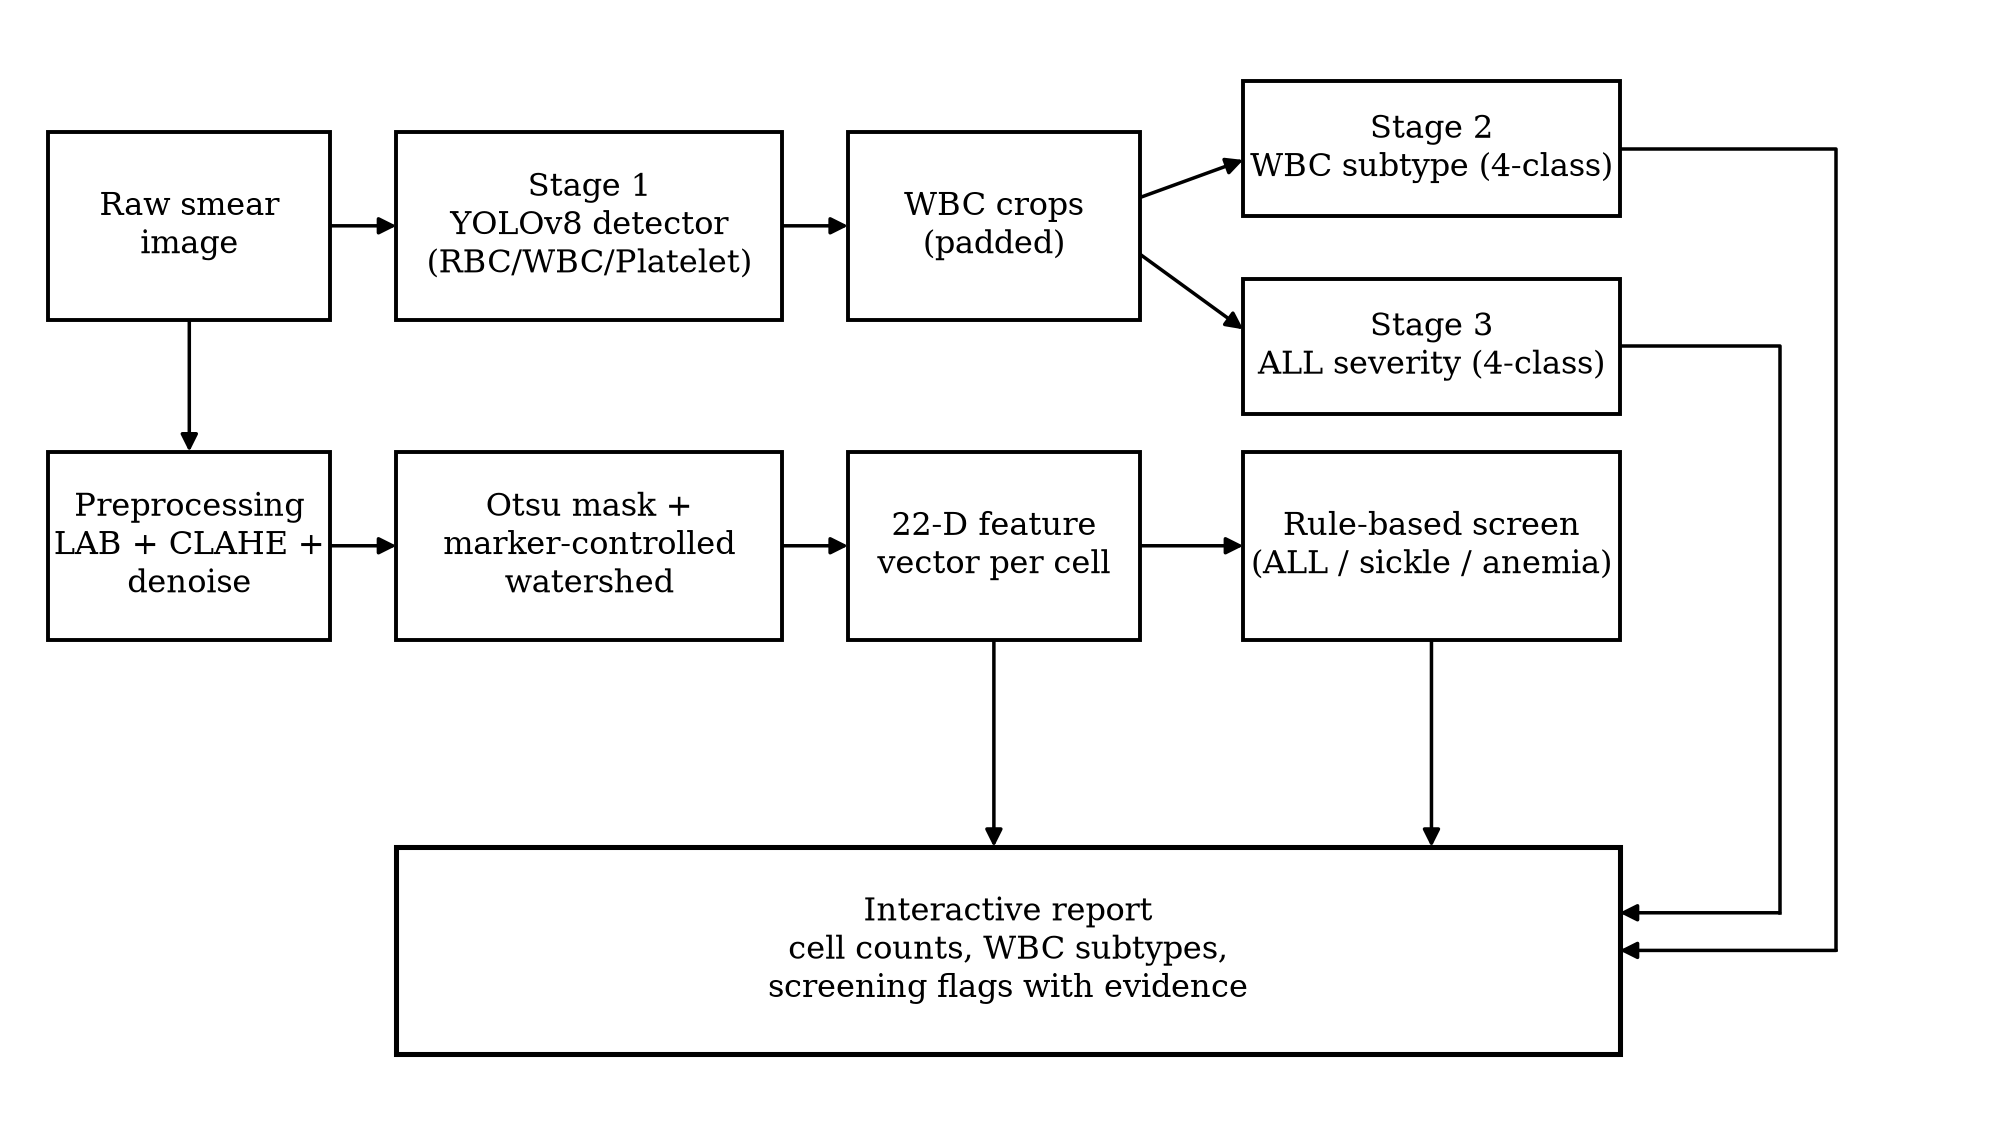
\includegraphics[width=0.95\linewidth]{figs/fig1_cascade.png}
\caption{End-to-end cascade: raw smear $\rightarrow$ Stage 1 detection $\rightarrow$ WBC crops $\rightarrow$ Stage 2 subtype / Stage 3 ALL-severity screening; preprocessing and watershed $\rightarrow$ features $\rightarrow$ rule-based screening.}
\label{fig:cascade}
\end{figure}

\begin{figure}[!t]
\centering
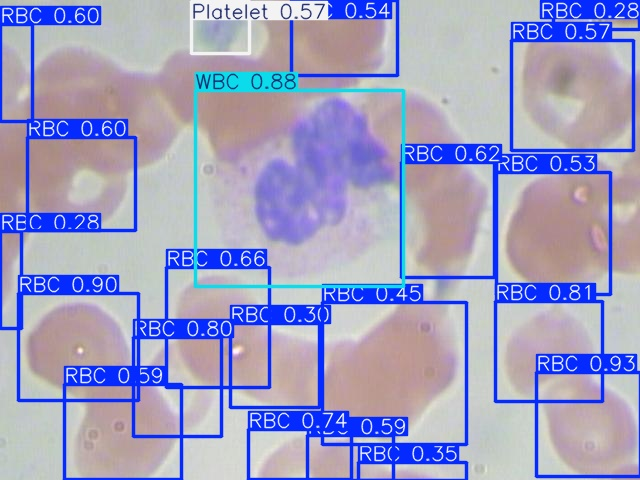
\includegraphics[width=0.95\linewidth]{figs/fig4_stage1_detection_sample.jpg}
\caption{Stage 1 YOLOv8 detections on a held-out BCCD test image (RBC/WBC/Platelet boxes with confidence scores).}
\label{fig:detsample}
\end{figure}

\begin{figure}[!t]
\centering
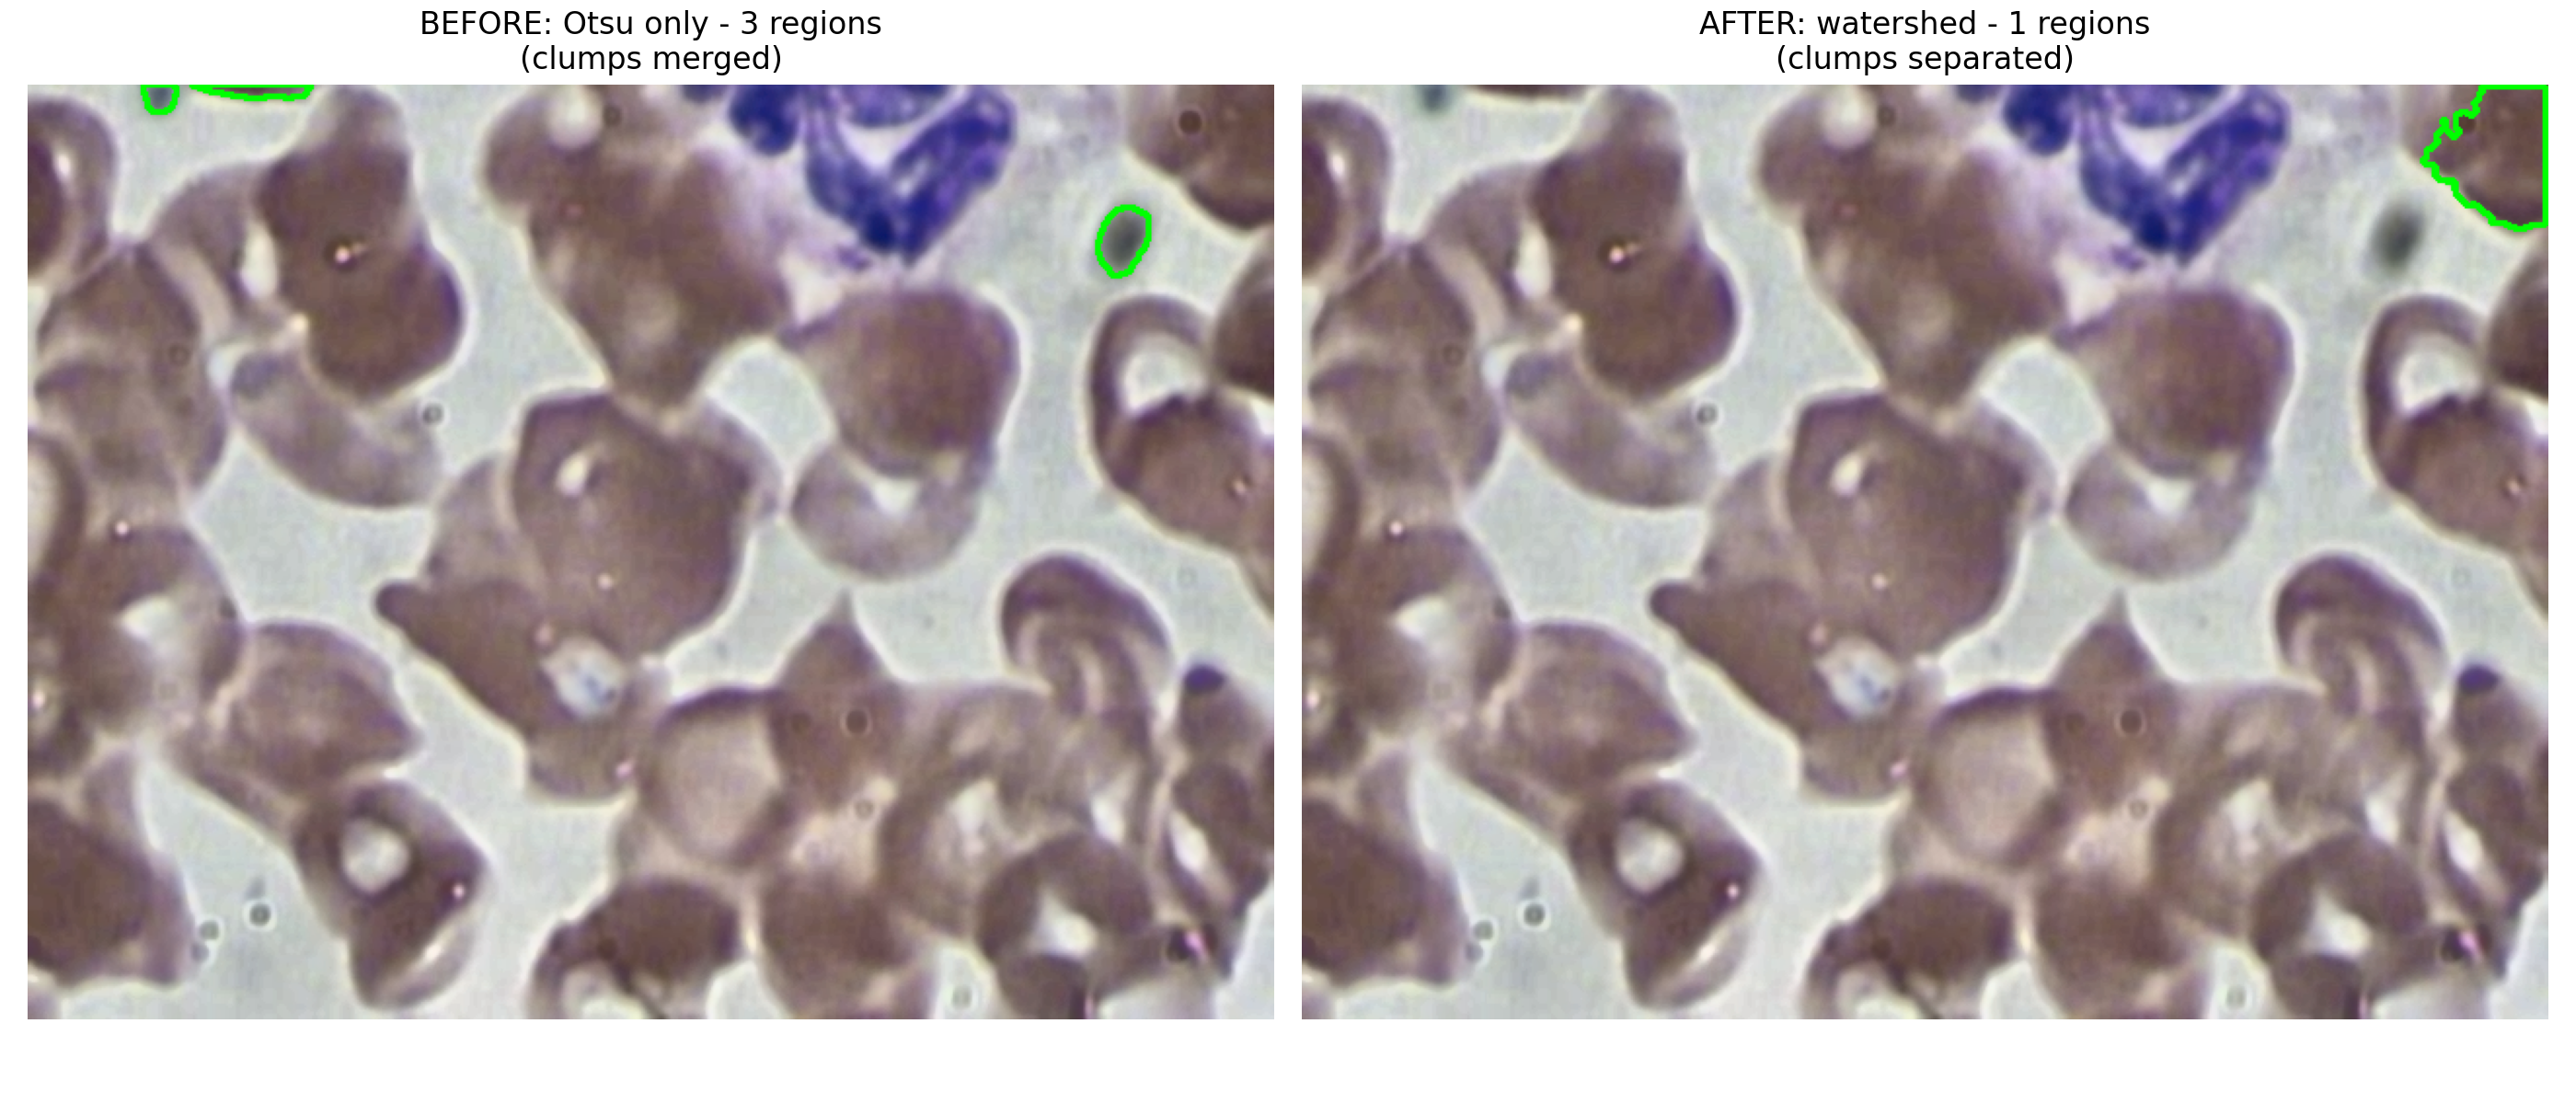
\includegraphics[width=0.95\linewidth]{figs/fig2_watershed.png}
\caption{Before-and-after watershed segmentation for a smear region containing touching RBCs.}
\label{fig:watershed}
\end{figure}

\begin{figure}[!t]
\centering
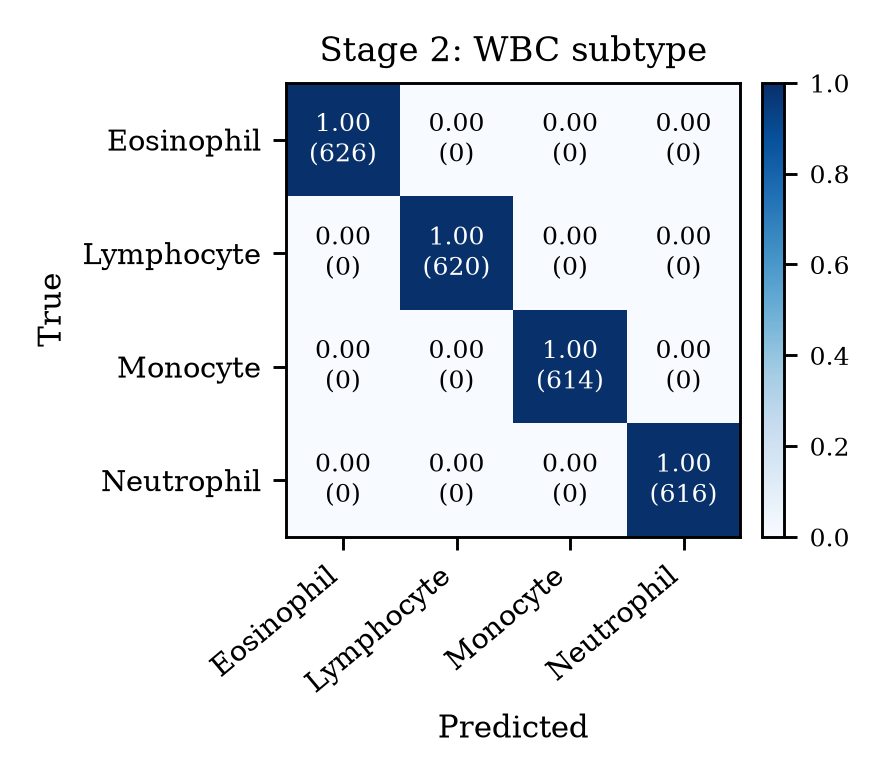
\includegraphics[width=0.48\linewidth]{figs/fig3a_stage2_confusion_matrix.png}\hfill
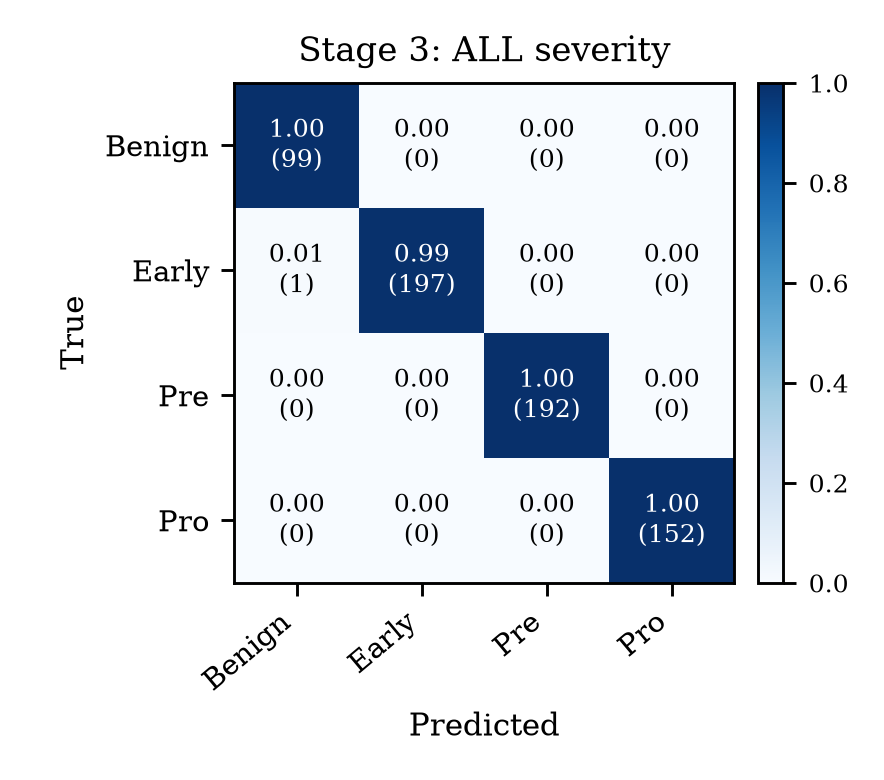
\includegraphics[width=0.48\linewidth]{figs/fig3b_stage3_confusion_matrix.png}
\caption{Row-normalized 4$\times$4 confusion matrices on the held-out split, with no background row/column: (a) Stage 2 WBC subtype (left); (b) Stage 3 ALL-severity screen (right). Cell labels show normalized recall with raw counts in parentheses.}
\label{fig:confmat}
\end{figure}

\begin{figure}[!t]
\centering
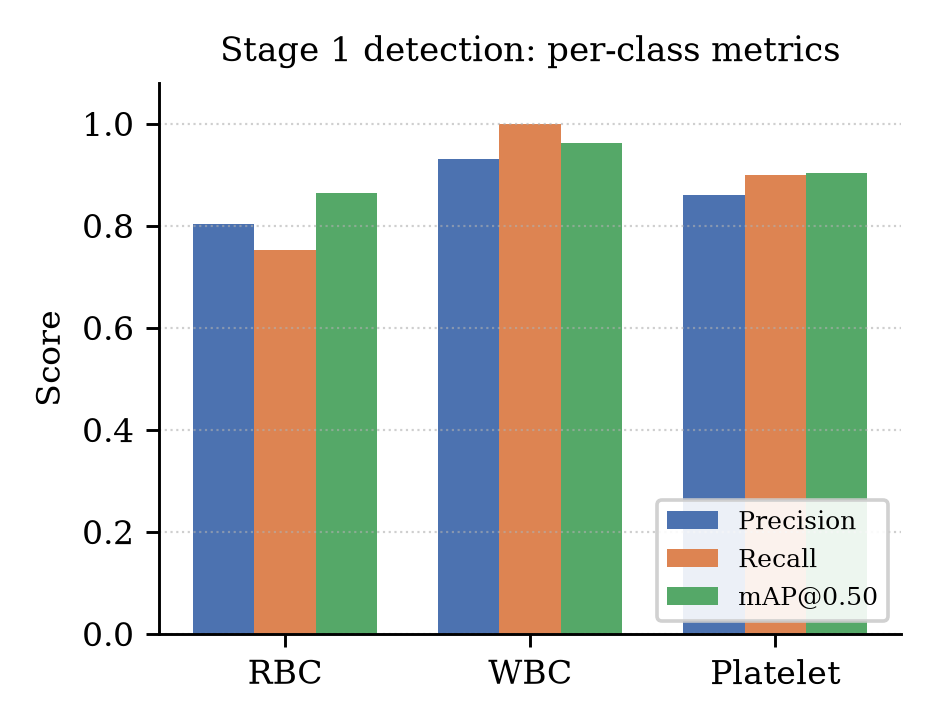
\includegraphics[width=0.95\linewidth]{figs/fig5_stage1_perclass_bars.png}
\caption{Stage 1 per-class precision, recall, and mAP@0.50 on the held-out test split.}
\label{fig:stage1bars}
\end{figure}

\begin{figure}[!t]
\centering
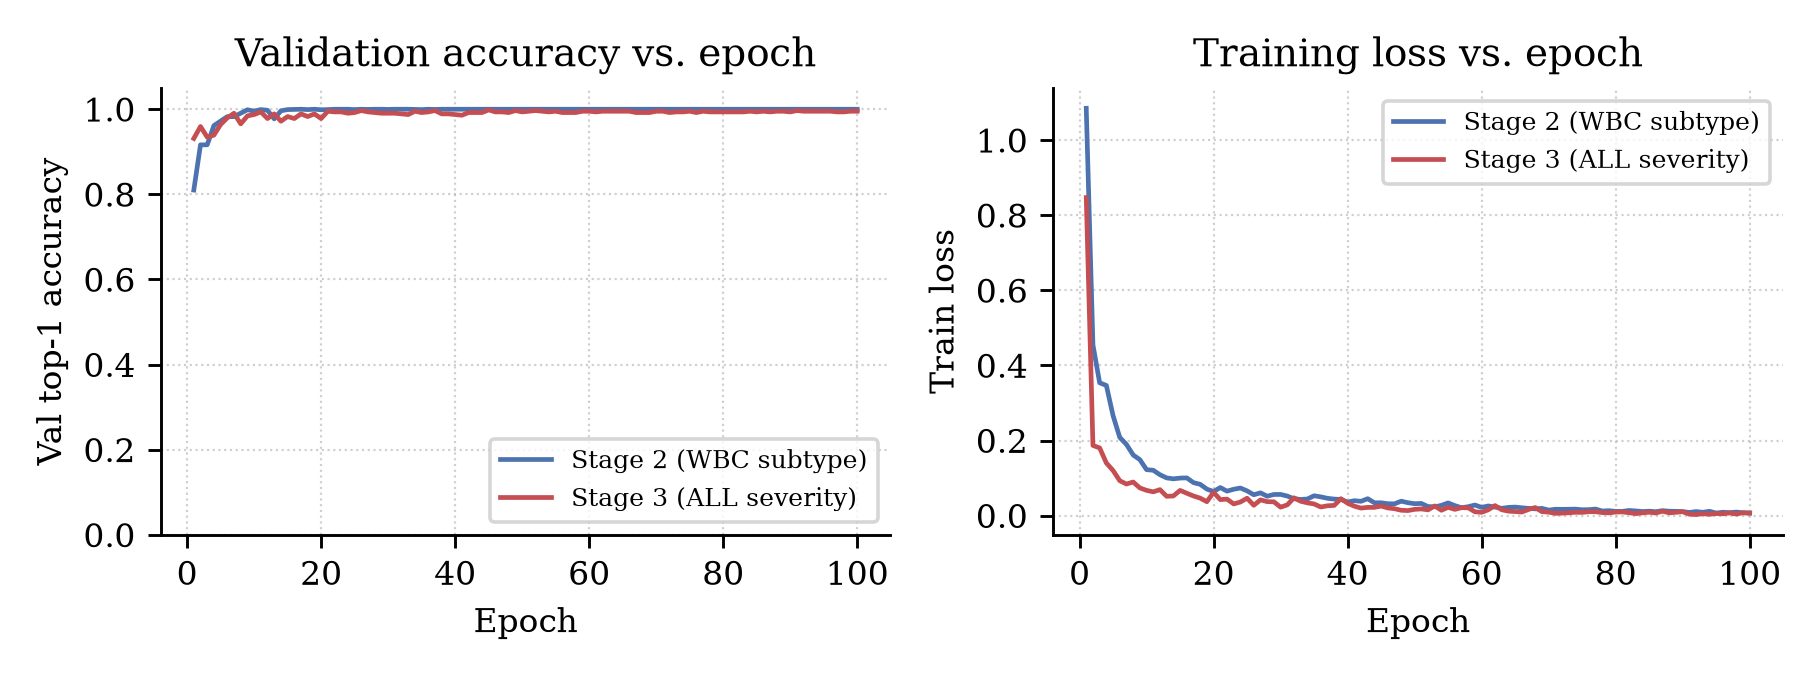
\includegraphics[width=0.95\linewidth]{figs/fig6_training_curves.png}
\caption{Stage 2 and Stage 3 training curves: held-out validation top-1 accuracy and training loss over 100 epochs.}
\label{fig:curves}
\end{figure}

\subsection{Interpretation}

Each confusion matrix should be interpreted class by class. Its diagonal entries are recalls after row normalization; off-diagonal entries identify subtype confusions. For Stage 3 (Table~\ref{tab:results}), the one error is a single Early sample predicted as Benign, giving Early a recall of 0.995 while every other class is perfect; MCC = 0.998 confirms this is a near-perfect, not merely accuracy-inflated, result. Stage 2 is exactly diagonal (MCC = 1.00) on 2{,}476 held-out crops.

These scores should not be read as evidence of clinical-grade performance. Three factors most likely explain them: (i) both classification datasets are curated, single-cell crops with consistent staining and framing, unlike a real peripheral-blood slide; (ii) the four WBC subtypes and four ALL severity classes are visually well-separated by colour and nuclear morphology even to the underlying compact YOLOv8n-cls backbone; and (iii) the held-out split, while verified leakage-free at the source-image level, is still drawn from the same acquisition batch and device as training data. A high accuracy accompanied by a high MCC here indicates the model has solved the dataset, not necessarily the general diagnostic task; Section V returns to this point. For Stage 1, mAP@0.50:0.95 (0.621) is noticeably lower than mAP@0.50 (0.910), indicating that RBC and platelet boxes are frequently correctly classified but loosely localized -- consistent with the more variable boundary of touching/overlapping RBCs (Fig.~\ref{fig:stage1bars}). The Stage 2/3 training curves (Fig.~\ref{fig:curves}) show validation accuracy plateauing by roughly epoch 20 with a smoothly decaying training loss and no divergence between the two, which is consistent with the models fitting the training distribution rather than an evaluation artefact such as a corrupted or overlapping split. All results remain limited to the chosen held-out split and must not be interpreted as clinical diagnostic accuracy.

\section{Discussion and Limitations}

The pipeline provides useful traceability: detections, crops, subtype predictions, cell measurements, and rule evidence can all be inspected. Its cascade also avoids pretending that the same dataset or model solves detection, subtype classification, and leukemia screening equally well.

Several limitations are important. First, the data are public, 8-bit images and may not represent scanner bit depth, staining protocols, devices, magnification, or the patient population found in clinical practice. Second, morphology thresholds and disorder scores are heuristic: the feature choices for sickle-cell and anemia screening follow established hematology references \cite{ref_bain,ref_who,ref_xu}, but the numerical cut-offs applied to those features require expert-labelled clinical validation before any diagnostic claim can be made. Third, a crop-level ALL-severity classifier trained on a curated single-cell dataset may face severe domain shift when applied to WBC crops taken from a different peripheral-smear acquisition pipeline; the 99.8--100\% held-out scores in Table~\ref{tab:results} should be read as evidence that the model fits these two specific public datasets very well, not as external validity. Fourth, segmentation quality cannot be reported as Dice without independent ground-truth masks; this study reports it qualitatively for that reason rather than substituting a proxy metric. Fifth, the nucleus-to-cell feature is reused as a stain-saturation pallor proxy for enucleated RBCs (Section III-C); this reinterpretation is documented but has not itself been validated against haemoglobin measurements. Finally, neither the UI nor the screening logic is a medical device or a substitute for hematologist review.

Future work should obtain expert-annotated masks and disease labels for sickle-cell and anemia so that the corresponding rule layers can be replaced or validated against ground truth, use patient- or source-group-independent (ideally cross-hospital) splits to stress-test the near-perfect Stage 2/3 scores reported here, report calibration and uncertainty, compare the cascade to baselines, and conduct multi-site validation.

\section{Conclusion}

This paper presents an interpretable blood-smear analysis prototype that combines YOLOv8 detection, WBC-crop classification, watershed segmentation, morphology features, and rule-based screening. The proposed verification layer matches evaluation metrics to each stage's task: detection is scored with IoU-based precision, recall, and mAP; both crop classifiers are scored with a genuine confusion matrix, per-class F1, and MCC; and segmentation is scored with Dice wherever ground truth permits. The project should be presented as a reproducible educational decision-support prototype whose two rule-based disease screens are grounded in cited hematological morphology rather than presented as validated diagnostic models. Its future value depends on leakage-resistant evaluation and clinically supervised validation rather than unsupported headline accuracy claims.

\section*{Declarations}

\textbf{Funding:} No external funding declared. Update if applicable.

\textbf{Conflict of interest:} The authors declare no conflict of interest.

\textbf{Ethics and intended use:} This project analyses public image data. It is not a diagnostic device and must not be used to make clinical decisions without qualified review.

\begin{thebibliography}{00}
\bibitem{ref_yolo} G. Jocher, A. Chaurasia, and J. Qiu, \emph{Ultralytics YOLO}, 2023. [Online]. Available: \url{https://docs.ultralytics.com/}
\bibitem{ref_clahe} K. Zuiderveld, ``Contrast limited adaptive histogram equalization,'' in \emph{Graphics Gems IV}, Academic Press, 1994, pp. 474--485.
\bibitem{ref_watershed} F. Meyer, ``Topographic distance and watershed lines,'' \emph{Signal Processing}, vol. 38, no. 1, pp. 113--125, 1994.
\bibitem{ref_matthews} B. W. Matthews, ``Comparison of the predicted and observed secondary structure of T4 phage lysozyme,'' \emph{Biochimica et Biophysica Acta}, vol. 405, no. 2, pp. 442--451, 1975.
\bibitem{ref_chicco} D. Chicco and G. Jurman, ``The advantages of the Matthews correlation coefficient (MCC) over F1 score and accuracy in binary classification evaluation,'' \emph{BMC Genomics}, vol. 21, no. 6, 2020.
\bibitem{ref_voc} M. Everingham, L. Van Gool, C. K. I. Williams, J. Winn, and A. Zisserman, ``The PASCAL Visual Object Classes (VOC) Challenge,'' \emph{International Journal of Computer Vision}, vol. 88, no. 2, pp. 303--338, 2010.
\bibitem{ref_dice} L. R. Dice, ``Measures of the amount of ecologic association between species,'' \emph{Ecology}, vol. 26, no. 3, pp. 297--302, 1945.
\bibitem{ref_bain} B. J. Bain, \emph{Blood Cells: A Practical Guide}, 5th ed. Chichester, U.K.: Wiley-Blackwell, 2015.
\bibitem{ref_who} World Health Organization, ``Haemoglobin concentrations for the diagnosis of anaemia and assessment of severity,'' Vitamin and Mineral Nutrition Information System, WHO/NMH/NHD/MNM/11.1, Geneva, 2011.
\bibitem{ref_xu} M. Xu, D. P. Papageorgiou, S. Z. Abidi, M. Dao, H. Zhao, and G. E. Karniadakis, ``A deep convolutional neural network for classification of red blood cells in sickle cell anemia,'' \emph{PLOS Computational Biology}, vol. 13, no. 10, e1005746, 2017.
\bibitem{ref_tomari} R. Tomari, W. N. W. Zakaria, M. M. A. Jamil, F. M. Nor, and N. F. N. Fuad, ``Computer aided system for red blood cell classification in blood smear image,'' \emph{Procedia Computer Science}, vol. 42, pp. 206--213, 2014.
\bibitem{ref_bccd} Shenggan, \emph{BCCD Dataset}, GitHub repository, 2018. [Online]. Available: \url{https://github.com/Shenggan/BCCD_Dataset}
\bibitem{ref_ghaderzadeh} M. Ghaderzadeh, M. Aria, A. Hosseini, F. Asadi, D. Bashash, and H. Abolghasemi, ``A fast and efficient CNN model for B-ALL diagnosis and its subtypes classification using peripheral blood smear images,'' \emph{International Journal of Intelligent Systems}, vol. 37, no. 8, pp. 5113--5133, 2022.
\end{thebibliography}

\end{document}
